\section{Performance of the Spherical Harmonics Analysis in Separating 0\nbb-decay from \B~Background.}
\label{sec:performance}

In this section we discuss factors that affect performance of the spherical harmonics analysis in separating
0\nbb~signal from \B~background events. We found that most separation comes from the first two multiple moments,
$l=0$ and $l=1$. However, according to Eq.~\ref{eq6}, higher multiple moments are needed for a better normalization of the 
power spectrum $S_l$. In the following we choose to calculate the power spectrum $s_l$ up to l=3 and
use only normalized variable $S_0$ and $S_1$, where the normalization is given by

\begin{eqnarray}
\label{eq7}
S_{0,1} = \frac{s_{0,1}}{\sum_{l=0}^{3} s_l}
\end{eqnarray}

As discussed below, a linear combination of $S_0$ and $S_1$ can be used to construct a single variable, $S_{01}$, that provides 
separation between signal and background in 1-D space. We show distributions of this variable $S_{01}$ to demonstrate
the separation between 0\nbb~and \B~events depending on a few key assumptions about the detector characteristics.


{\it {\bf The following paragraph needs to be moved to intro and maybe re-phrased. }
Since the goal of this paper is to describe the technique of spherical harmonics analysis for separating
different event topologies relevant for 0\nbb-decay searches in a generic liquid scintillator detector, we intentionally refrain from any 
quantitative estimates on the improvements in sensitivity to 0\nbb~decay. The actual improvements in sensitivity due to spherical 
harmonics analysis would depend on various details of a given experimental setup. Therefore, we believe that detailed quantitative 
sensitivity studies are more appropriate in the context of a particular 0\nbb~decay experiment which is beyond the scope of this paper.
}

\subsection{Central events with no uncertainty on the vertex position}

We start evaluating the performance of the spherical harmonics analysis by looking at events that originate at the center
of the detector and by assuming perfect reconstruction of the event vertex position. For such events, a time cut of 33.5~ns on 
the PE arrival time can be applied to obtain early an PEs sample which contains a high fraction of Cherenkov PEs. The default QE and 100\% 
photo-coverage are used in the simulation.

A comparison of $S_0$ and $S_1$ distributions for 0\nbb-decay signal and \B~background events is shown in Fig.~\ref{fig:S_vs_energy}.
Both variables provide a noticeable separation between signal and background. We also note that in the energy range of interest, 
the $S_l$'s do not strongly depend on the energy deposited in the detector, which makes information contained in the normalized power 
spectrum complimentary to the energy measurements. Spherical harmonics analysis can thus be used as an additional handle for
background suppression at the end point of the 0\nbb-decay energy spectrum.

\begin{figure*}[h]
\centering
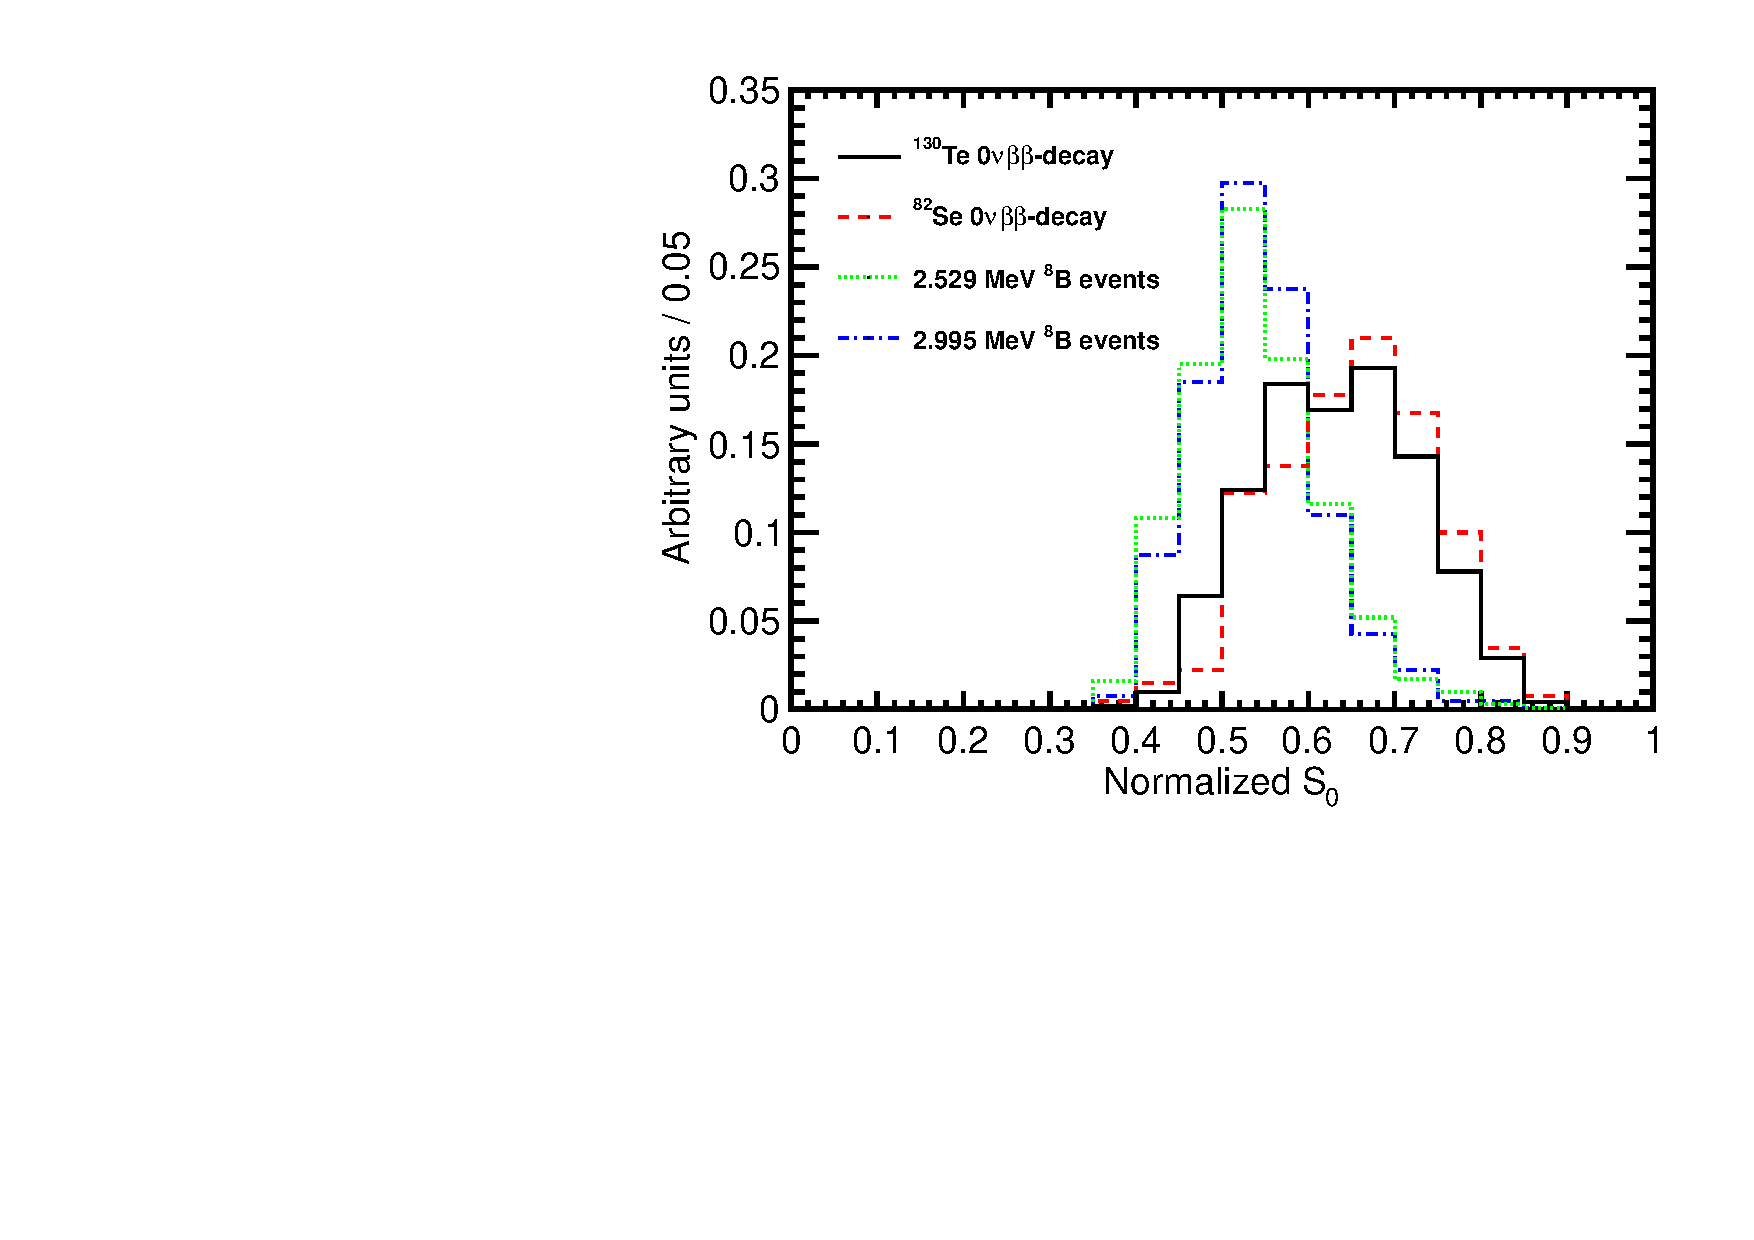
\includegraphics[width=0.49\textwidth]{hS0.pdf}
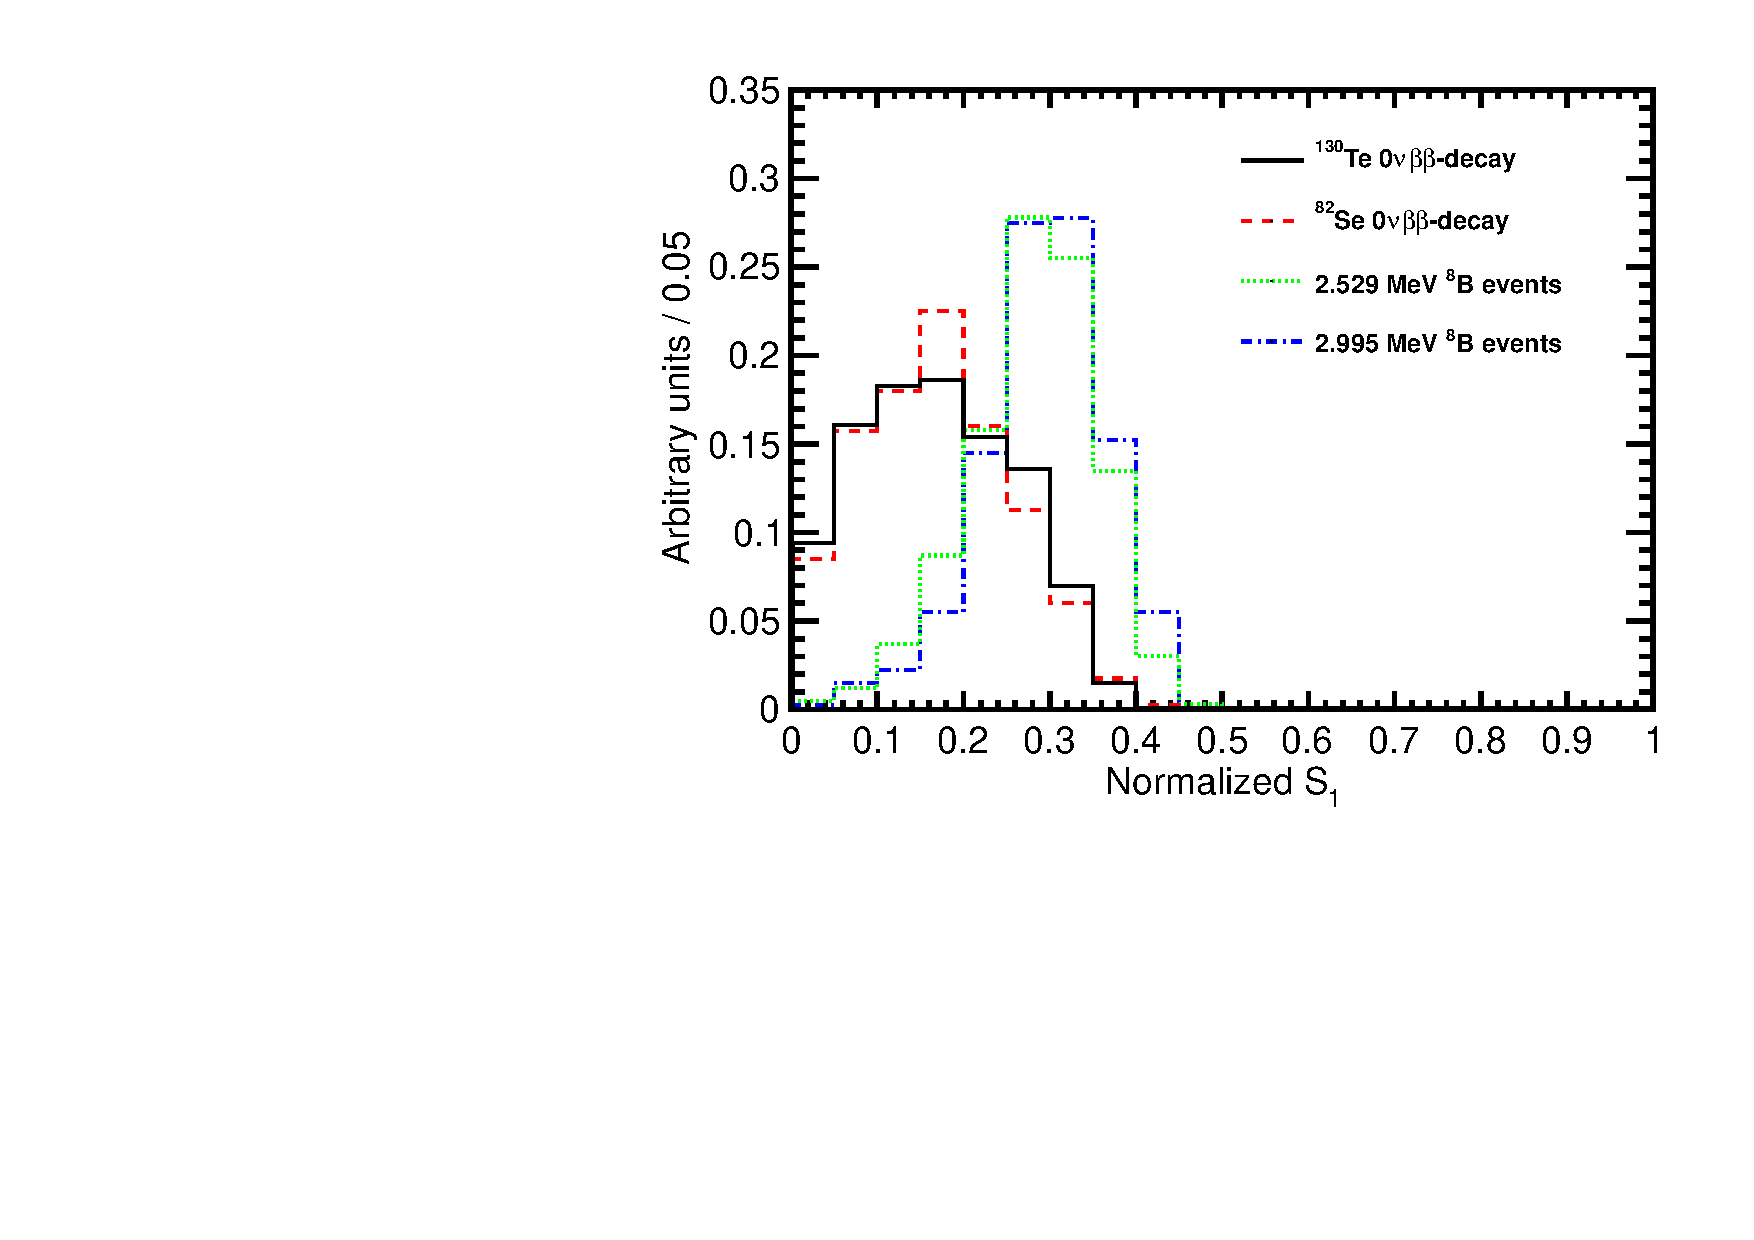
\includegraphics[width=0.49\textwidth]{hS1.pdf}
\caption{$S_0$ (\emph{left}) and $S_1$ (\emph{right}) distributions for 1000 simulated 0\nbb-decay signal and \B~background events.
  Two different isotopes are compared, $^{130}$Te and $^{82}$Se. Corresponding kinetic energies of \B~single electrons are
  2.53 MeV and 3.00 MeV. Central events assuming perfect reconstruction of vertex position. Time cut of 33.5~ns on the PE arrival time is
  applied. The default QE and 100\% photo-coverage is used in the simulation.}
\label{fig:S_vs_energy}
\end{figure*}

Left panel in Fig.~\ref{fig:SL_Te_33p5ns_center} compares scatter plots of the first two components of the power spectrum, 
$S_0$ and $S_1$, for signal and background. In order to optimize separation between $^{130}$Te and $^{8}$B
events, a linear combination of variables $S_0$ and $S_1$ is constructed as follows. 

First, a linear fit, $S_0$ = $A \cdot S_1 + B$, of all points on the scatter plot is performed as shown by the dashed 
line in the left panel in Fig.~\ref{fig:SL_Te_33p5ns_center}. Then a 1-D variable $S_{01}$ is defined as
$S_{01} = S_1 \cdot cos(\theta) + S_0 \cdot sin(\theta)$, where $tan(\theta)$=$A$. The right-hand panel in Fig.~\ref{fig:SL_Te_33p5ns_center}
compares distributions of $S_{01}$ for 0\nbb-decay signal and \B~background. These 1-D histograms for $S_{01}$ represent the
projection of the points on the scatter plot onto the fitted line. 
%We use the distribution of the variable $S_{01}$ as a figure of merit
%for signal/background separation. 
To quantify the separation between the signal and background we calculate the area of the overlap in the $S_{01}$ distributions, 
$I_{overlap}$. There is no separation if $I_{overlap}$=1 and there is a 100\% separation if $I_{overlap}$=0. 
%We also calculate the distance between the mean values of each $S_{01}$ distribution relative to their root mean 
%squares (RMS), $\epsilon = \frac{ \overline{S_{01}^{bkg}} - \overline{S_{01}^{sig}} } {\sqrt{ RMS_{bkg}^2 + RMS_{sig}^2 }}$, where
%$\overline{S_{01}^{bkg}}$ and $\overline{S_{01}^{sig}}$ are the mean values, $RMS_{bkg}$ and $RMS_{sig}$
%are the RMS values of background and signal $S_{01}$ distribution respectively. In the following we use the ratio 
%$\frac{\epsilon}{I}$ as a measure for the separation between the signal and backgrdound.

Figure~\ref{fig:SL_Te_33p5ns_center} demonstrates that spherical harmonics analysis potentially brings extra separation power, which 
is in addition to the energy measurements. The overlap between signal and background is $I_{overlap}$=0.52.
%The separation $\frac{\epsilon}{I} = \frac{0.915}{0.521} = 1.76$.


\begin{figure*}[h]
  \centering
  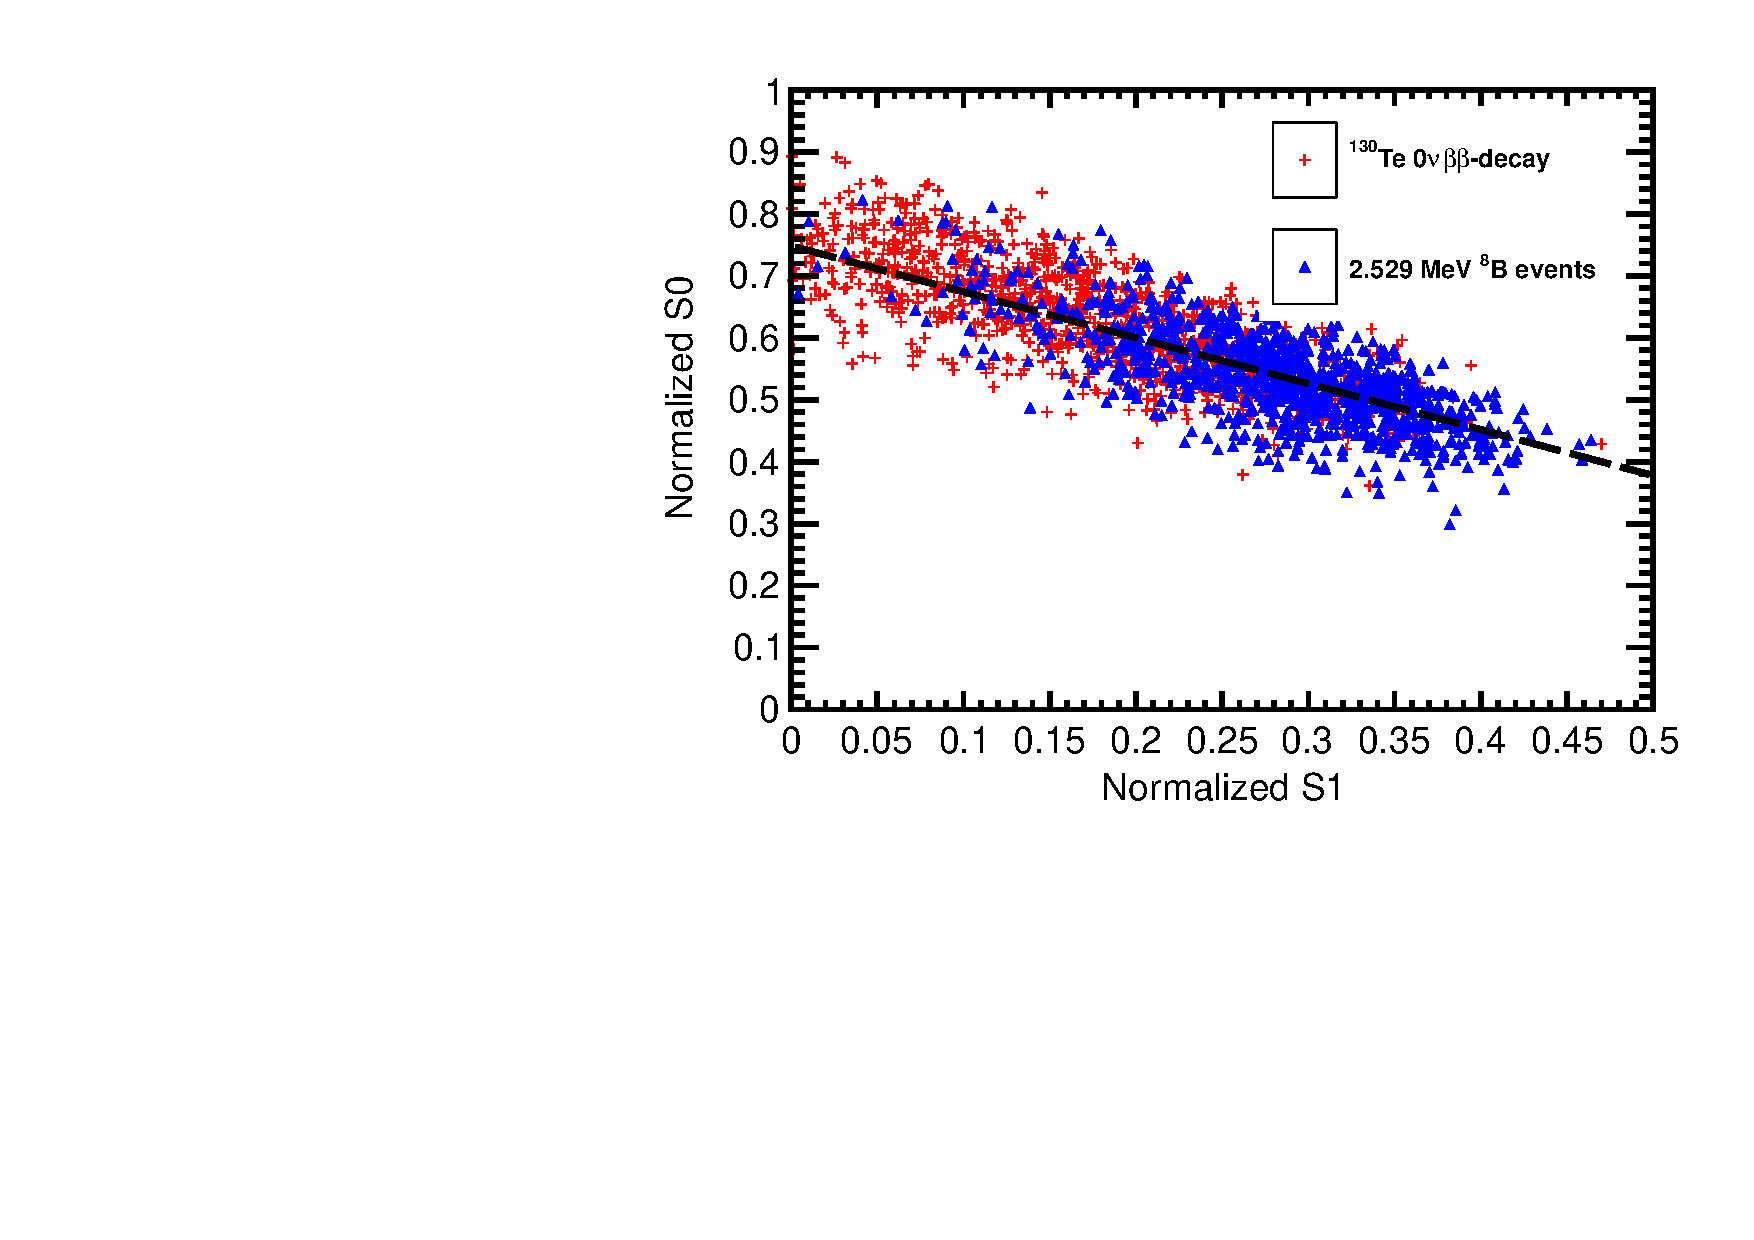
\includegraphics[width=0.49\textwidth]{hS0vsS1_Te130_1el_allLight_VtxSmear0cm_VtxShiftX0cm_33p5ns_center.pdf}
%  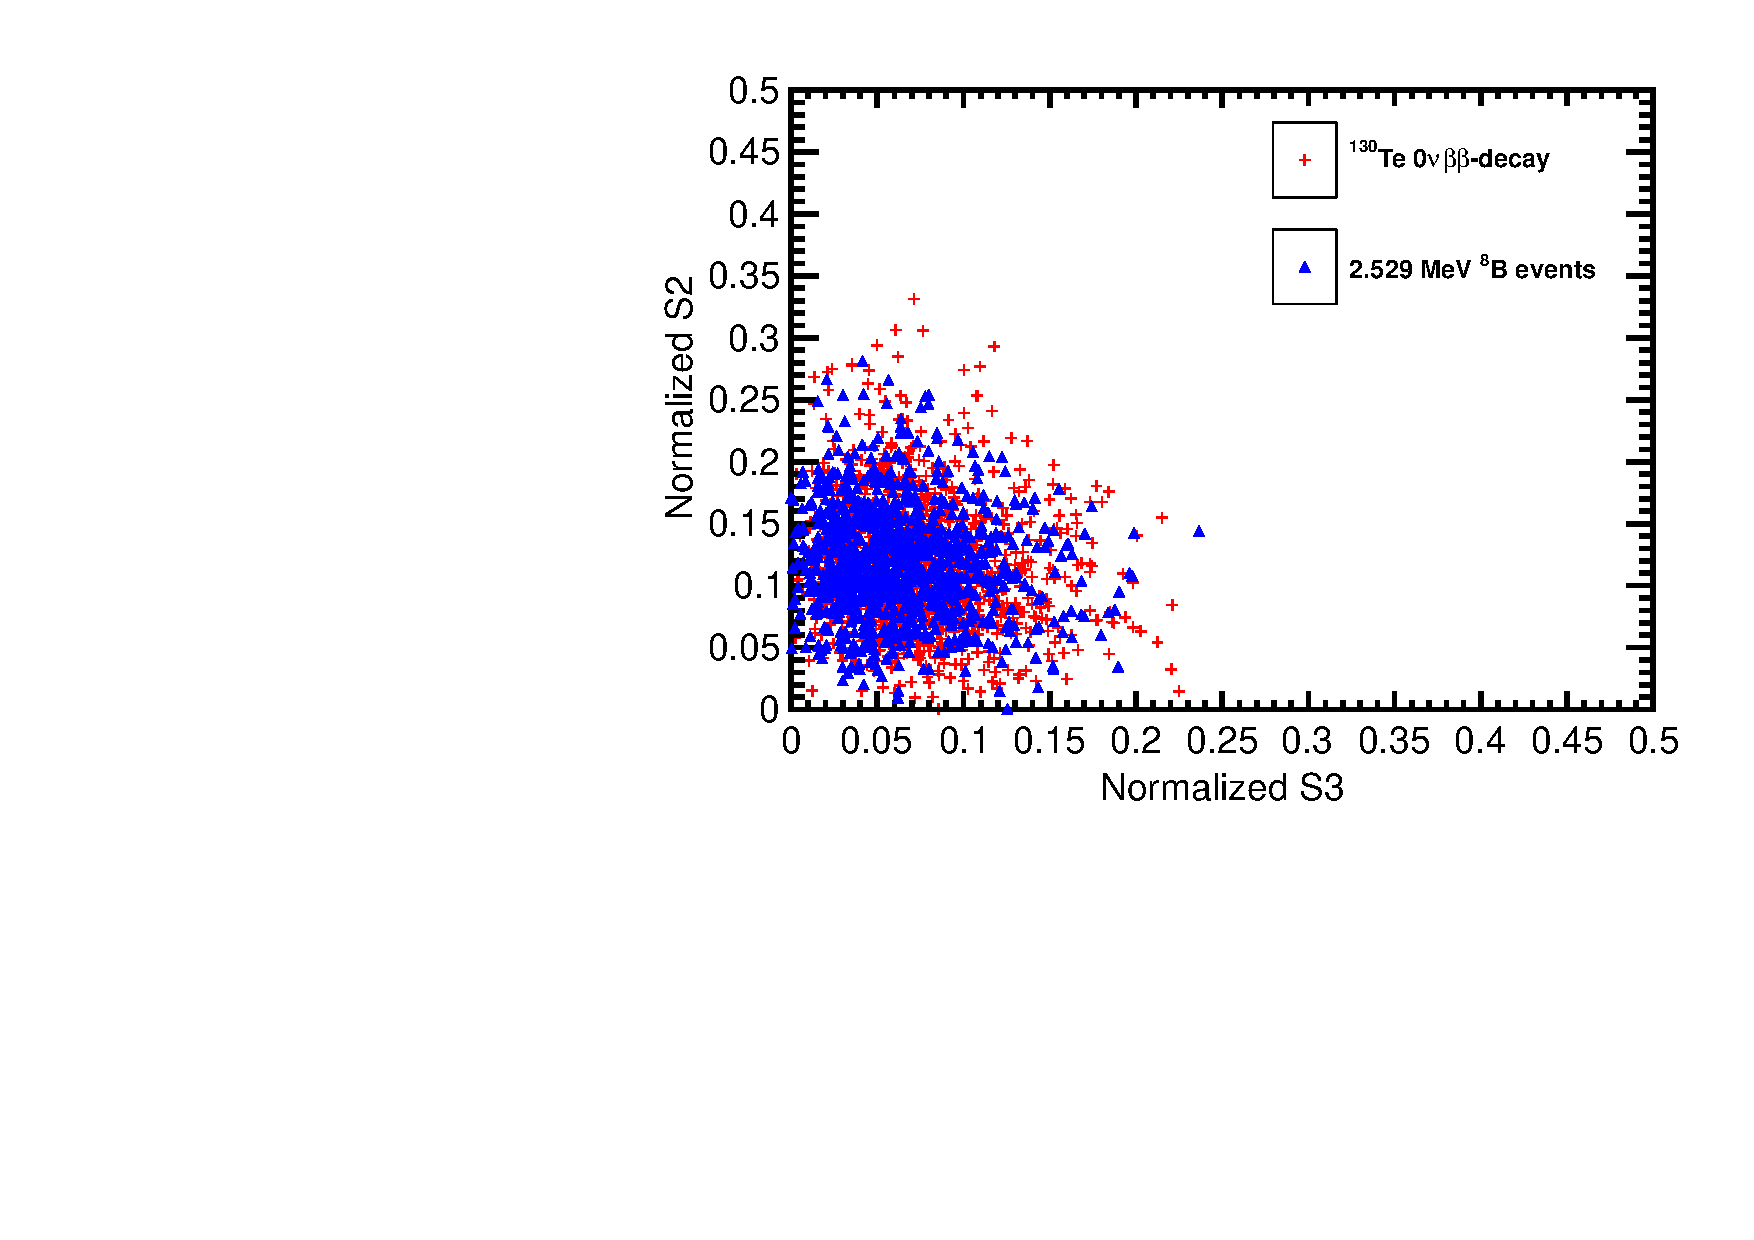
\includegraphics[width=0.49\textwidth]{hS2vsS3_Te130_1el_allLight_VtxSmear0cm_VtxShiftX0cm_33p5ns_center.pdf}
  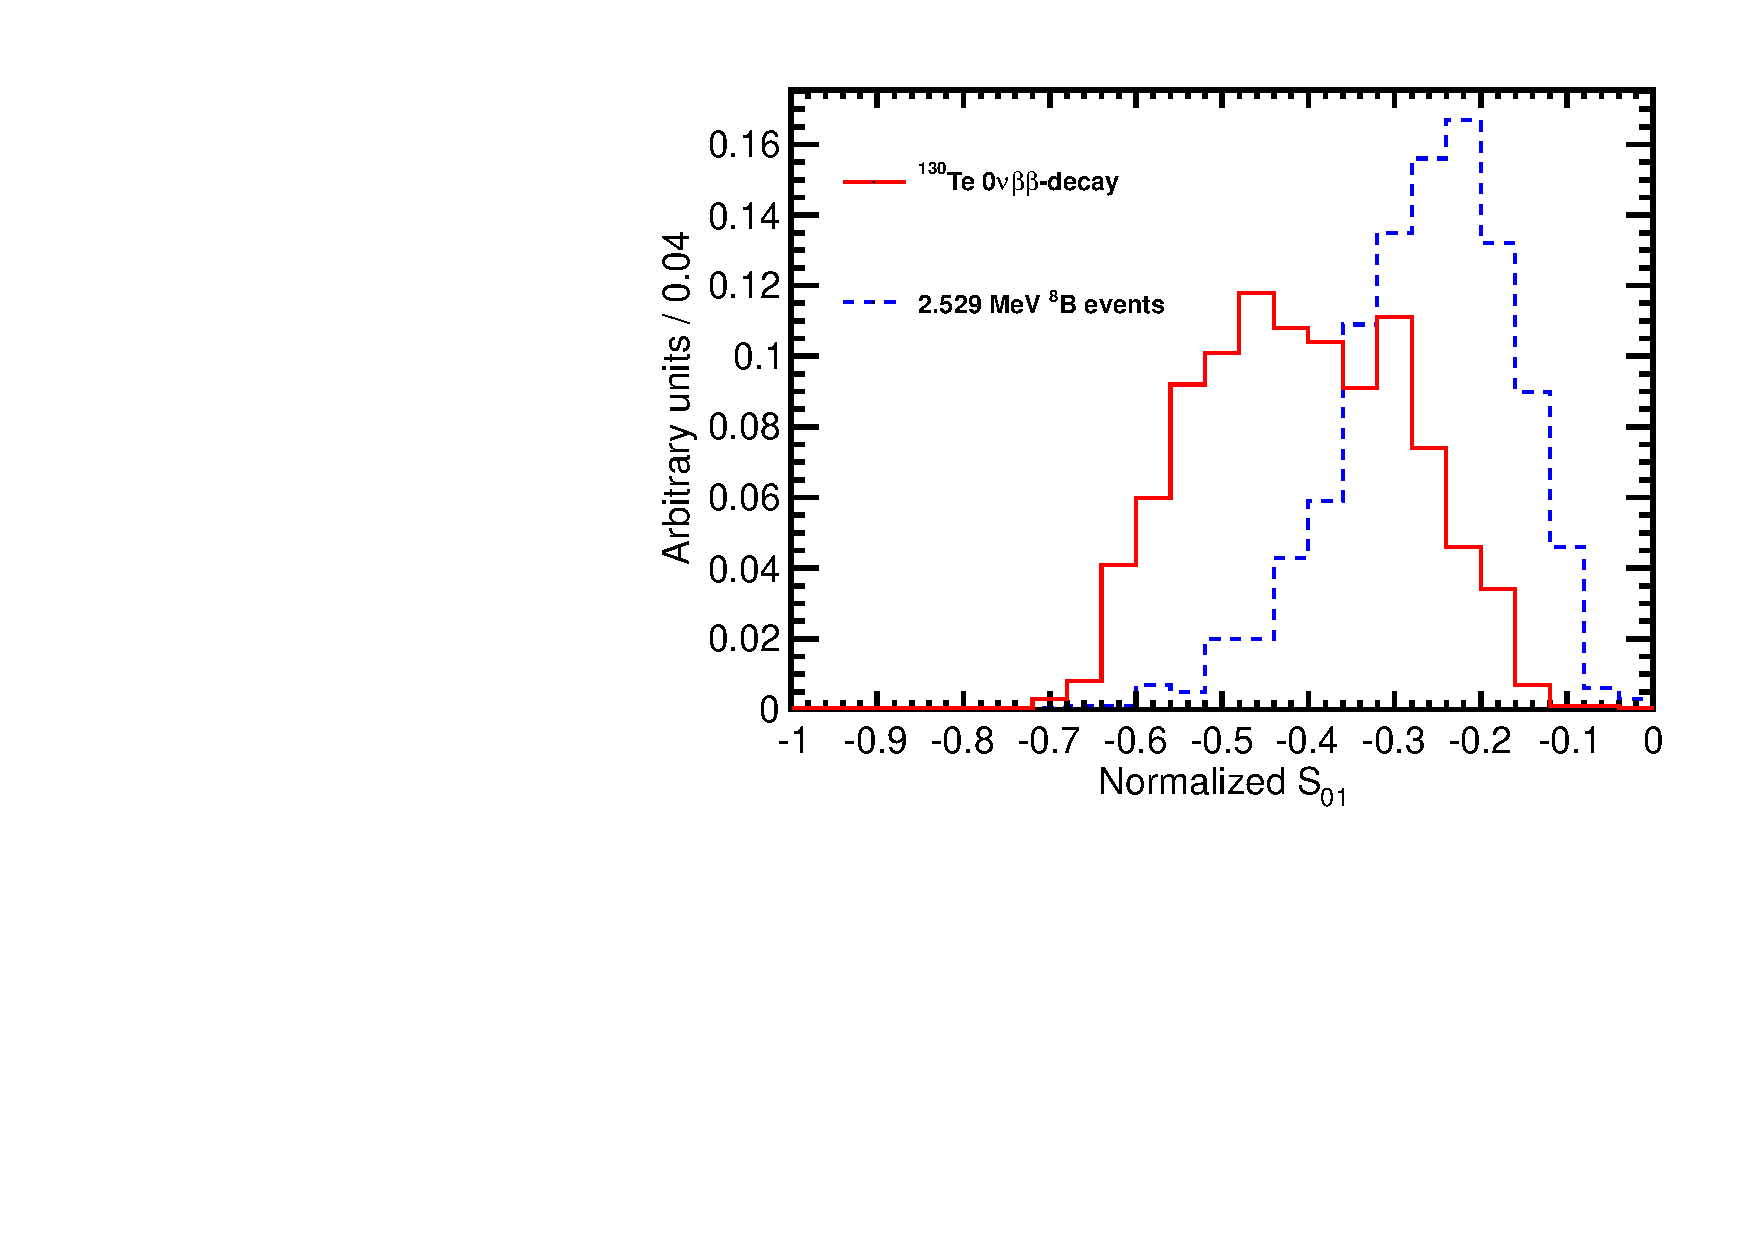
\includegraphics[width=0.49\textwidth]{hS01_allLight_VtxSmear0cm_VtxShiftX0cm_33p5ns_center.pdf}
  \caption{\emph{Left:} Scatter plot of $S_0$ versus $S_1$ for a simulation of 1000 signal (\emph{red crosses}) and background 
    (\emph{blue triangles}) events.
    Central events assuming perfect reconstruction of vertex position. Time cut of 33.5~ns on the PE arrival time is
    applied. The default QE and 100\% photo-coverage is used in the simulation.
    Black dashed line corresponds to a linear fit to define 1-D variable $S_{01}$ (see text for details).
    \emph{Right:} Comparison of the $S_{01}$ distribution between signal (\emph{red solid line}) and background (\emph{blue dashed line}).
    $I_{overlap}$=0.52.}
\label{fig:SL_Te_33p5ns_center}
\end{figure*}

%separation = 0.915454
%overlap = 0.521

\subsection{Experimental challenges: chromatic dispersion and vertex resolution}

So far only events at the center of the detector have been considered. Precise vertex reconstruction has been also assumed. 
Here we discuss performance of the spherical harmonics analysis for events that originate throughout the whole fiducial volume
of the detector and that also have limited vertex reconstruction precision.

Selection of the early PE sample using the absolute time cut of 33.5~ns that has been applied to central events relies on the fact that, 
within the uncertainty on electron track length, all photons travel the same distance before reaching the surface of the detector. 
PEs with early measured time correspond mostly to Cherenkov photons because of the delay in the scintillation process and longer 
wavelength of the Cherenkov light. 

Since in general the vertex is not at the center of the detector, a uniform absolute time cut on the photon arrival time is no longer 
effective in selecting Cherenkov photons. In the case of an off-center vertex, even significantly delayed scintillation photons can
reach the side of the detector that is closer to the vertex much earlier than Cherenkov photons traveling to the opposite side of the 
detector. The time cut thus has to take into account the total distance traveled by each individual photon.

We found that a differential time cut defined as $\Delta t=t^{phot}_{measured} - t^{phot}_{predicted}<$1~ns selects photons with a 
sufficient fraction being Cherenkov photons. However, when this differential time cut is applied, 
chromatic dispersion and vertex resolution significantly reduce the Cherenkov/scintillation light separation in the early PE sample.
and therefore, reduce discrimination power of the spherical harmonics analysis. In the following we describe both effects and 
propose solutions to mitigate their influence on the spherical harmonics analysis.

%\subsubsection{Chromatic dispersion}
The predicted time, 
$t^{phot}_{predicted}=l/v^{phot}$, depends on the distance, $l$, traveled by the photon and the velocity of the photon, 
$v^{phot}$.  Since the wavelength information is not available for a given PE, we use an average index of refraction, $n$, 
and define the photon velocity as $v^{phot} = c/n$. This uncertainty on the photon velocity makes the differential time cut less 
effective in separating Cherenkov light from scintillation light. 

%Poor Cherenkov/scintillation light separation reduces the effectiveness of the spherical harmonics analysis. For each event topology 
%spherical harmonics power spectrum is mostly determined by distinct distributions of Cherenkov photons. At the same time scintillation 
%photons represent uniform background noise for event topology reconstruction.


%\subsubsection{Vertex resolution} 
%Imprecise knowledge of the vertex position affects the spherical harmonics analysis in two ways. First, s
Similarly to the effect of chromatic 
dispersion, the vertex uncertainty makes the differential time cut less efficient in separating Cherenkov and scintillation light. 
An uncertainty on the vertex position leads to an uncertainty on the photon predicted travel time, $t^{phot}_{predicted}$, which in turn
increases the probability to mix scintillation and Cherenkov light in the early PE sample.

%Second, 
In addition, in the case of single electron event topology, a small error in vertex reconstruction could cause a large effect on the 
normalized power spectrum of spherical harmonics.

The early PE sample of the single electron topology typically has a strong asymmetry due
to preferential directionality of Cherenkov PEs that are selected together with uniformly distributed scintillation PEs. 
A mis-reconstructed vertex introduces an artificial asymmetry in the selection of scintillation PEs. Vertex shifts parallel to the direction of 
the electron track have the largest effect compared to the shifts in the transverse direction. 

If a vertex is shifted in the direction opposite to the track of the electron, the differential time cut selects more scintillation 
photons that are emitted in the direction of the electron track. Therefore scintillation photons would enhance forward asymmetry of the early PE
sample, which in turn, would move $S_1$ to higher values\footnote{In general, $S_1$ component of the
spherical harmonics power spectrum is higher for asymmetric distributions and lower for symmetric distributions (e.g., compare back-to-back
and single electron topologies in Fig.~\ref{fig:ThreeTopologies_Display_5MeV}). Moreover, $S_1=$~0 for a distribution with perfect symmetry
with respect to the center of the sphere.}.

If a vertex is shifted in the same direction as the direction of the electron, the differential time cut selects more scintillation
photons that are emitted in the direction opposite to the electron track. Therefore, the asymmetry of Cherenkov PEs would be counter
balanced by scintillation PEs, which in turn, would move $S_1$ to lower values.


\subsection{Events in a fiducial volume with an uncertainty on the vertex position}
We found that in our default detector model the separation power of the spherical harmonics analysis is reduced to X when
chromatic dispersion and vertex resolution are taken into account.

We simulated 1000 signal and background events that have their verticies uniformly distributed within a fiducial volume of $R<3$~m, 
where $R$ is the distance between the event vertex and the center of the detector. To implement an uncertainty on the vertex 
reconstruction we apply a 3~cm smearing around the actual vertex position for each simulated event. The smearing is done along $x$, $y$, 
and $z$ directions with three independent Gaussian distributions of the same width, $\sigma_x = \sigma_y = \sigma_z =$3~cm.

Figure~\ref{fig:SL_Te_SmearX3cm_momDT1ns_rndVtx_3p0m} shows the performance of the spherical harmonics analysis under these more realistic 
assumptions. The overlap between signal and background is $I_{overlap}$=0.79, which means that the separation is 52\% worse than in 
an idealized scenario shown in Fig.~\ref{fig:SL_Te_33p5ns_center}.
The spherical harmonics analysis brings little
separation between signal and background in our default detector model after the chromatic dispersion and
vertex resolution are taken into account. However, properties of the liquid scintillator can be adjusted to improve 
the performance of the spherical harmonics analysis. In the folowing we show that a single change in the scintillation rise time
improves the separation.
%restores most of the separation power that was shown previously in Fig.~\ref{fig:SL_Te_33p5ns_center}.



\begin{figure*}[h]
  \centering
  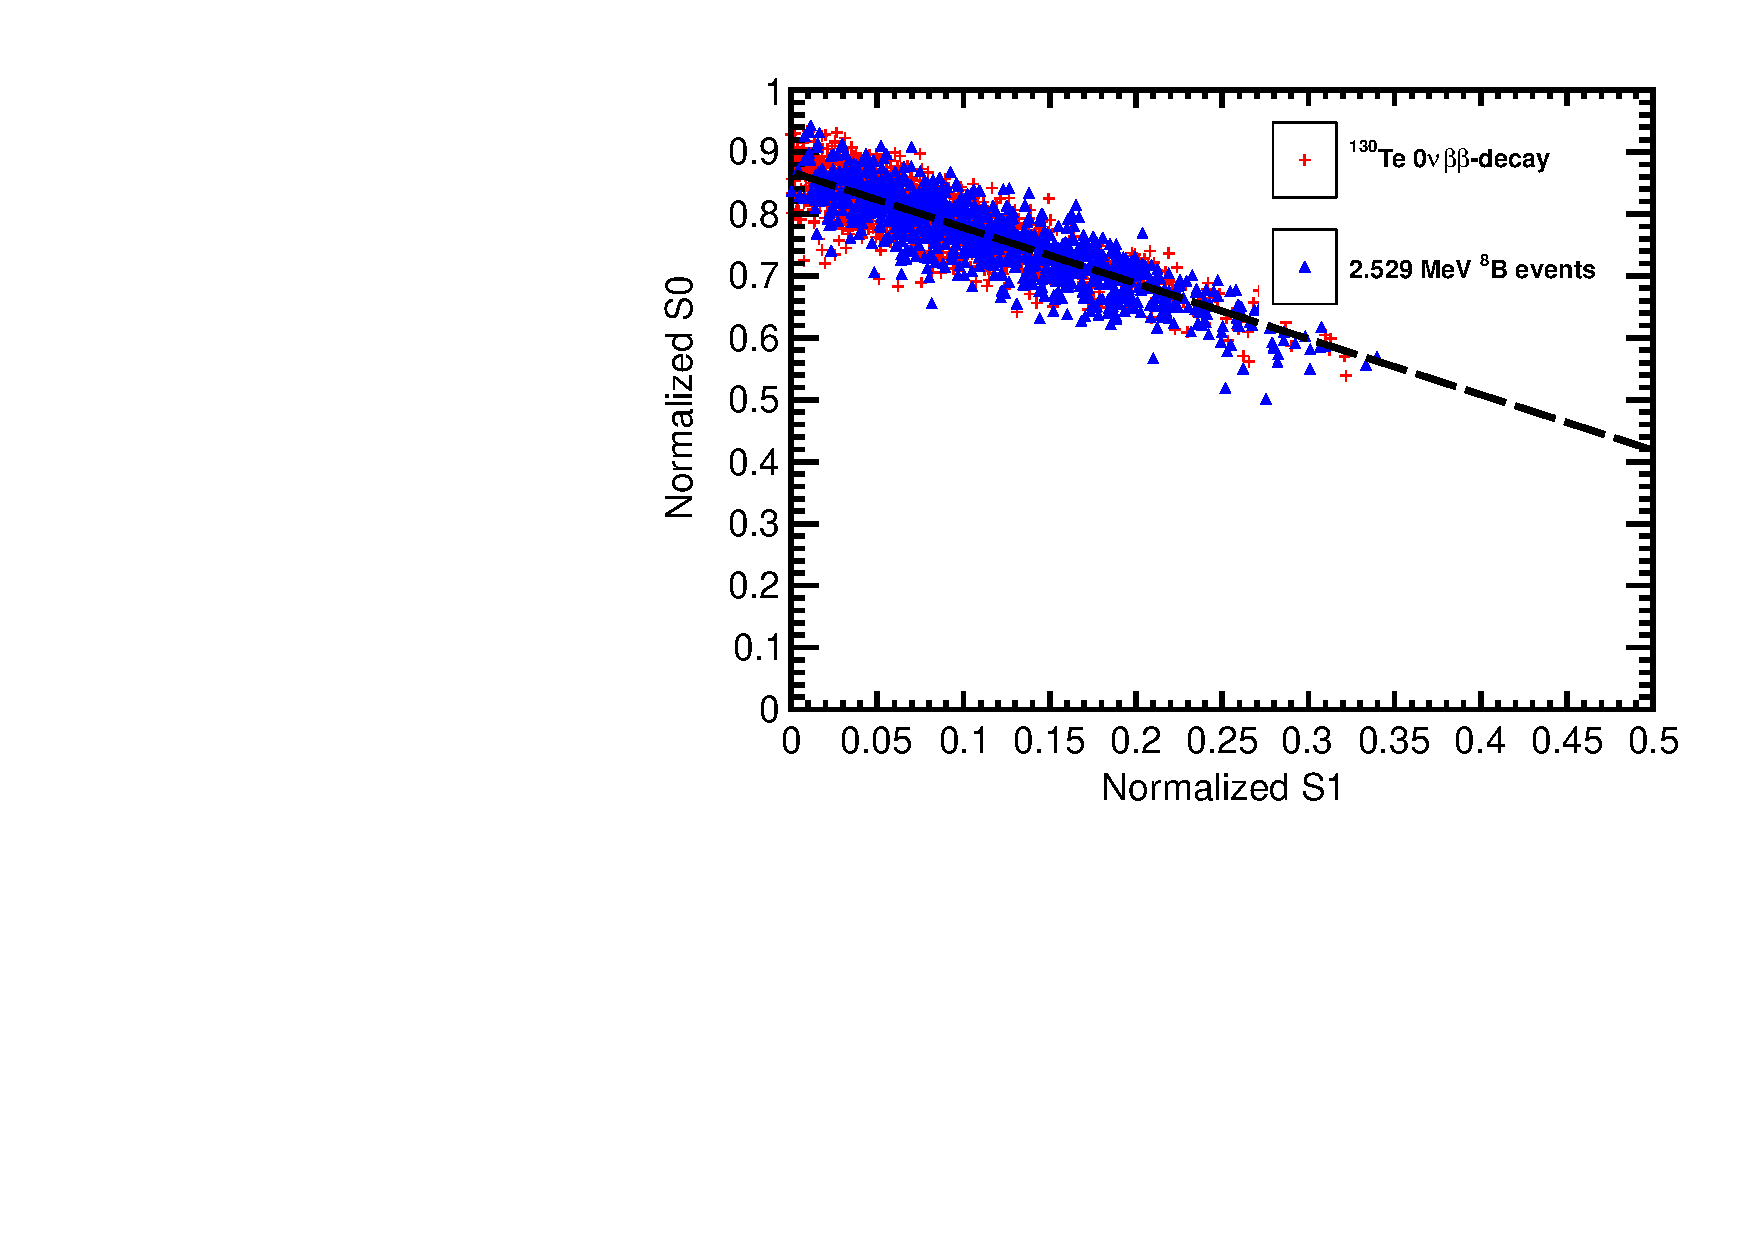
\includegraphics[width=0.49\textwidth]{hS0vsS1_Te130_1el_allLight_VtxSmear3cm_VtxShiftX0cm_momDT1p0ns_rndVtx_3p0mSphere.pdf}
  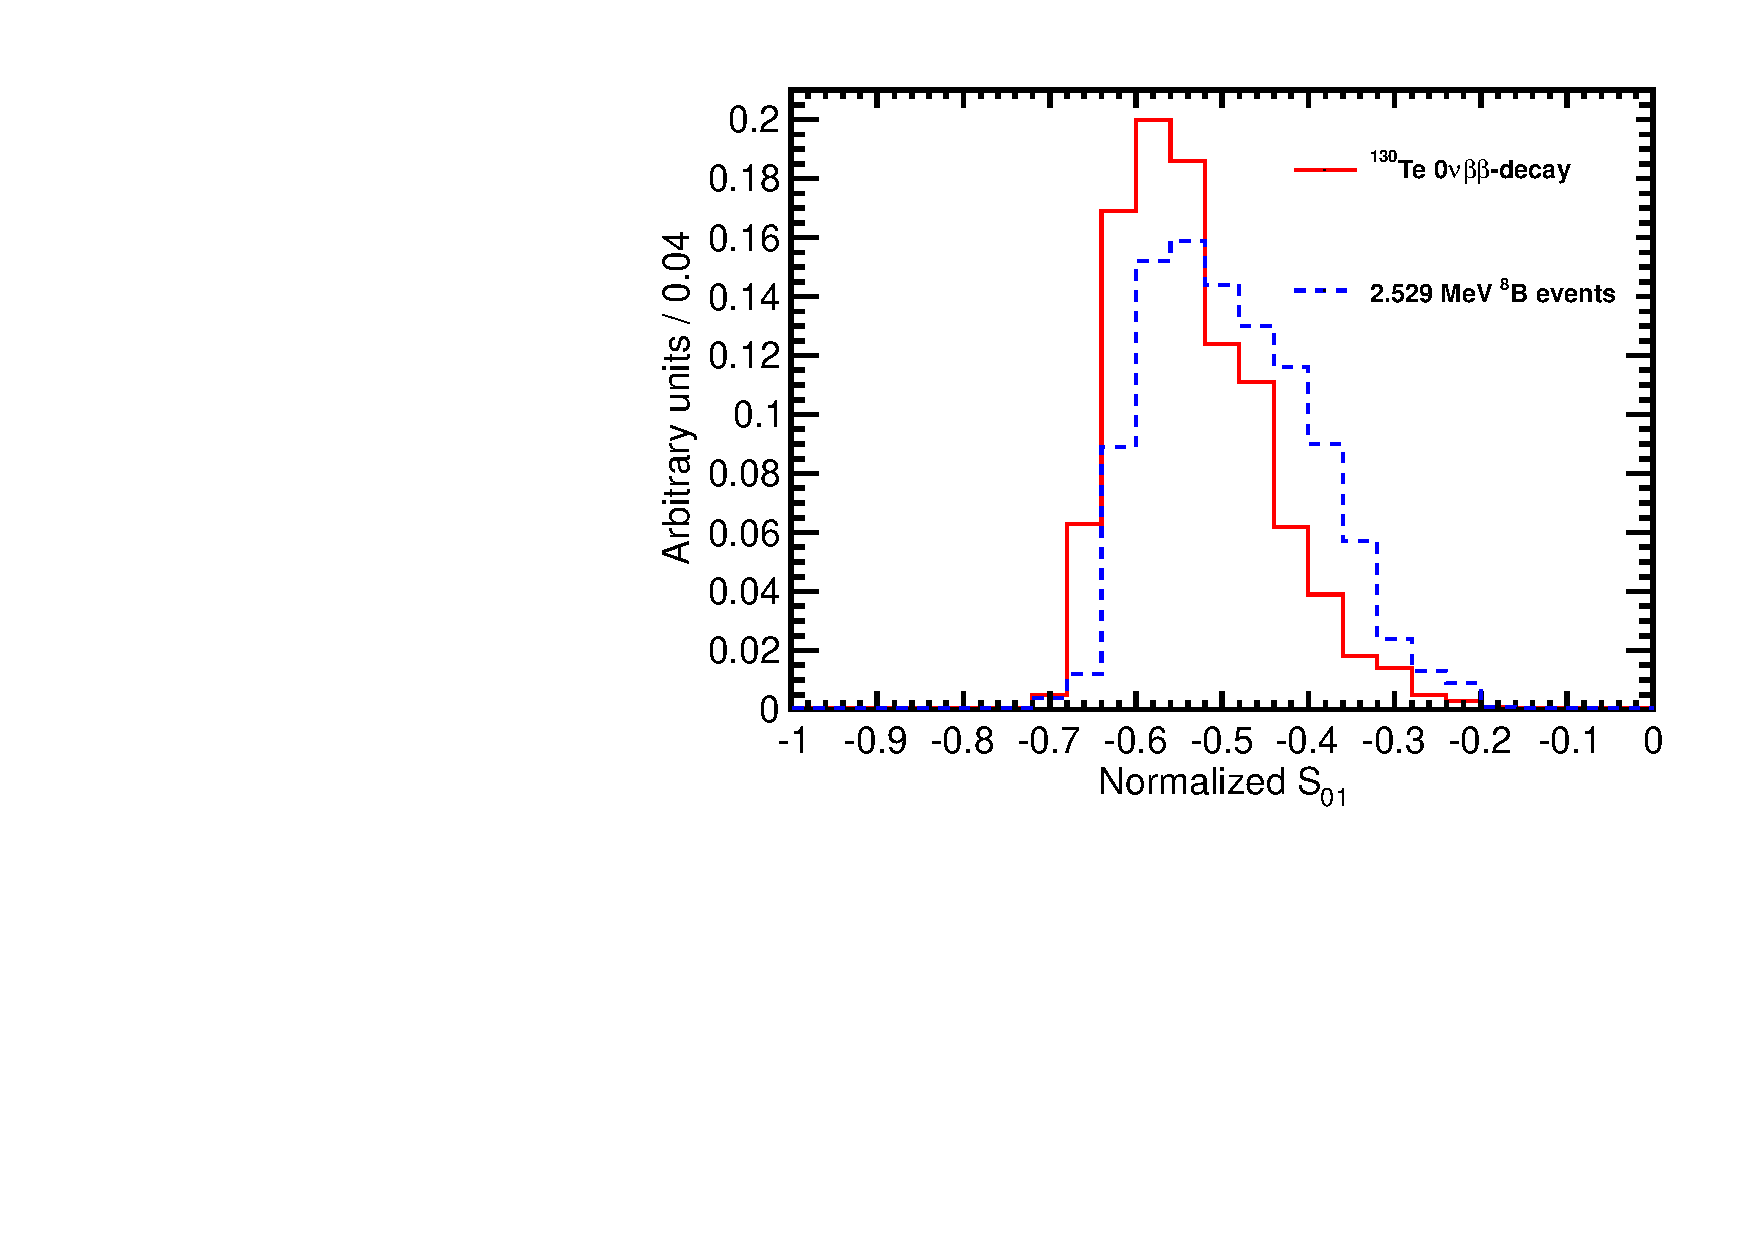
\includegraphics[width=0.49\textwidth]{hS01_allLight_VtxSmear3cm_VtxShiftX0cm_momDT1p0ns_rndVtx_3p0mSphere.pdf}
  \caption{\emph{Left:} Scatter plot of $S_0$ versus $S_1$ for a simulation of 1000 signal (\emph{red crosses}) and background
    (\emph{blue triangles}) events. Event verticies are uniformly distributed within the fiducial volume, $R<3$~m.
    Vertex is smeared with 3~cm resolution. Differential cut of
    $\Delta t=t^{phot}_{measured} - t^{phot}_{predicted}<$1~ns is applied to select early PE sample.
    The default QE and 100\% photo-coverage is used in the simulation.
    Black dashed line corresponds to a linear fit to define 1-D variable $S_{01}$ (see text for details).
    \emph{Right:} Comparison of the $S_{01}$ distribution between signal (\emph{red solid line}) and background (\emph{blue dashed line}).
    $I_{overlap}$=0.79.}
\label{fig:SL_Te_SmearX3cm_momDT1ns_rndVtx_3p0m}
\end{figure*}

%separation = 0.357271
%overlap = 0.793


\subsection{Importance of the liquid scintillator properties}
Strong dependence on the vertex resolution can be addressed by choosing a liquid scintillator mixture with a more delayed emission 
of scintillation light with respect to Cherenkov light. With a larger delay in scintillation light, a higher fraction of Cherenkov light 
can be maintained in the early PE sample even if a photon track length is mis-reconstructed due to imprecise reconstruction of the vertex 
position. In addition, if the fraction of scintillation light is small compared to Cherenkov light, the distortions in the uniformity of 
the scintillation PE due to shifted reconstructed vertex position does not significantly affect spherical harmonics power spectrum.

While our default detector model assumes scintillation rise time of $\tau_r=$1~ns, scintillation rise time up to $\tau_r=$7~ns can 
be achieved (see Ref.~\ref{Mingfang_slow_rise_time}). As a test we increased the scintillation rise time parameter to $\tau_r=$5~ns in 
our detector model and repeated spherical harmonics analysis on 0\nbb-decay and \B~events that are uniformly distributed within the fiducial 
volume and that have each vertex smeared with 3~cm resolution. All other parameters are kept the same.
Figure ~\ref{fig:SL_Te_SmearX3cm_momDT1ns_rndVtx_3p0m_SciRT5p0ns} shows the 
result of that test. The overlap between signal and background is $I_{overlap}$=0.64, which means that the separation is 23\% worse than in
an idealized scenario shown in Fig.~\ref{fig:SL_Te_33p5ns_center} and 23\% better than in the default detector model shown in 
Fig.~\ref{fig:SL_Te_SmearX3cm_momDT1ns_rndVtx_3p0m}.

We conclude that a rise time of $\tau_r=$5~ns provides sufficient delay between
Cherenkov and scintillation light to make spherical harmonics analysis a potentially useful technique to separate 
0\nbb-decay signal from \B~background.

\begin{figure*}[h]
  \centering
  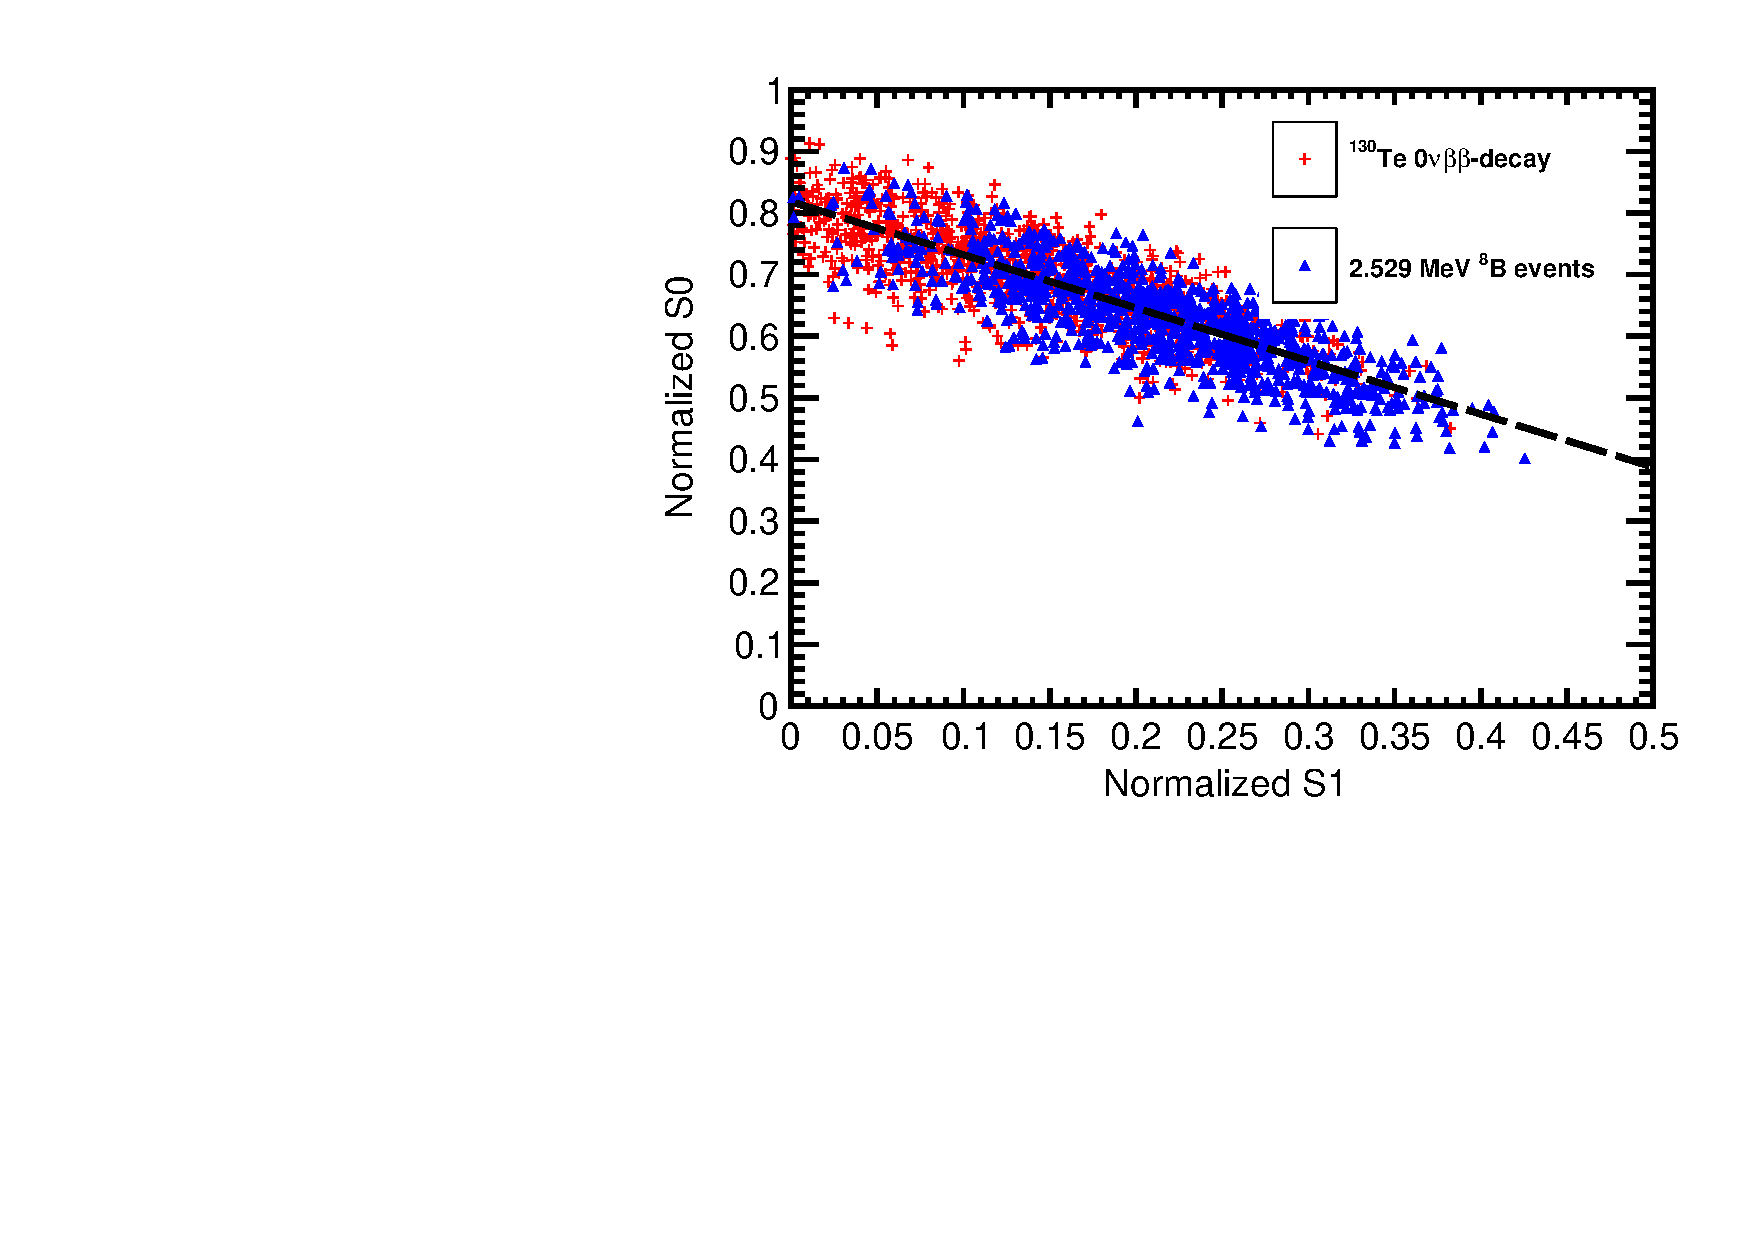
\includegraphics[width=0.49\textwidth]{hS0vsS1_Te130_1el_allLight_VtxSmear3cm_VtxShiftX0cm_momDT1p0ns_rndVtx_3p0mSphere_SciRT5p0ns} 
  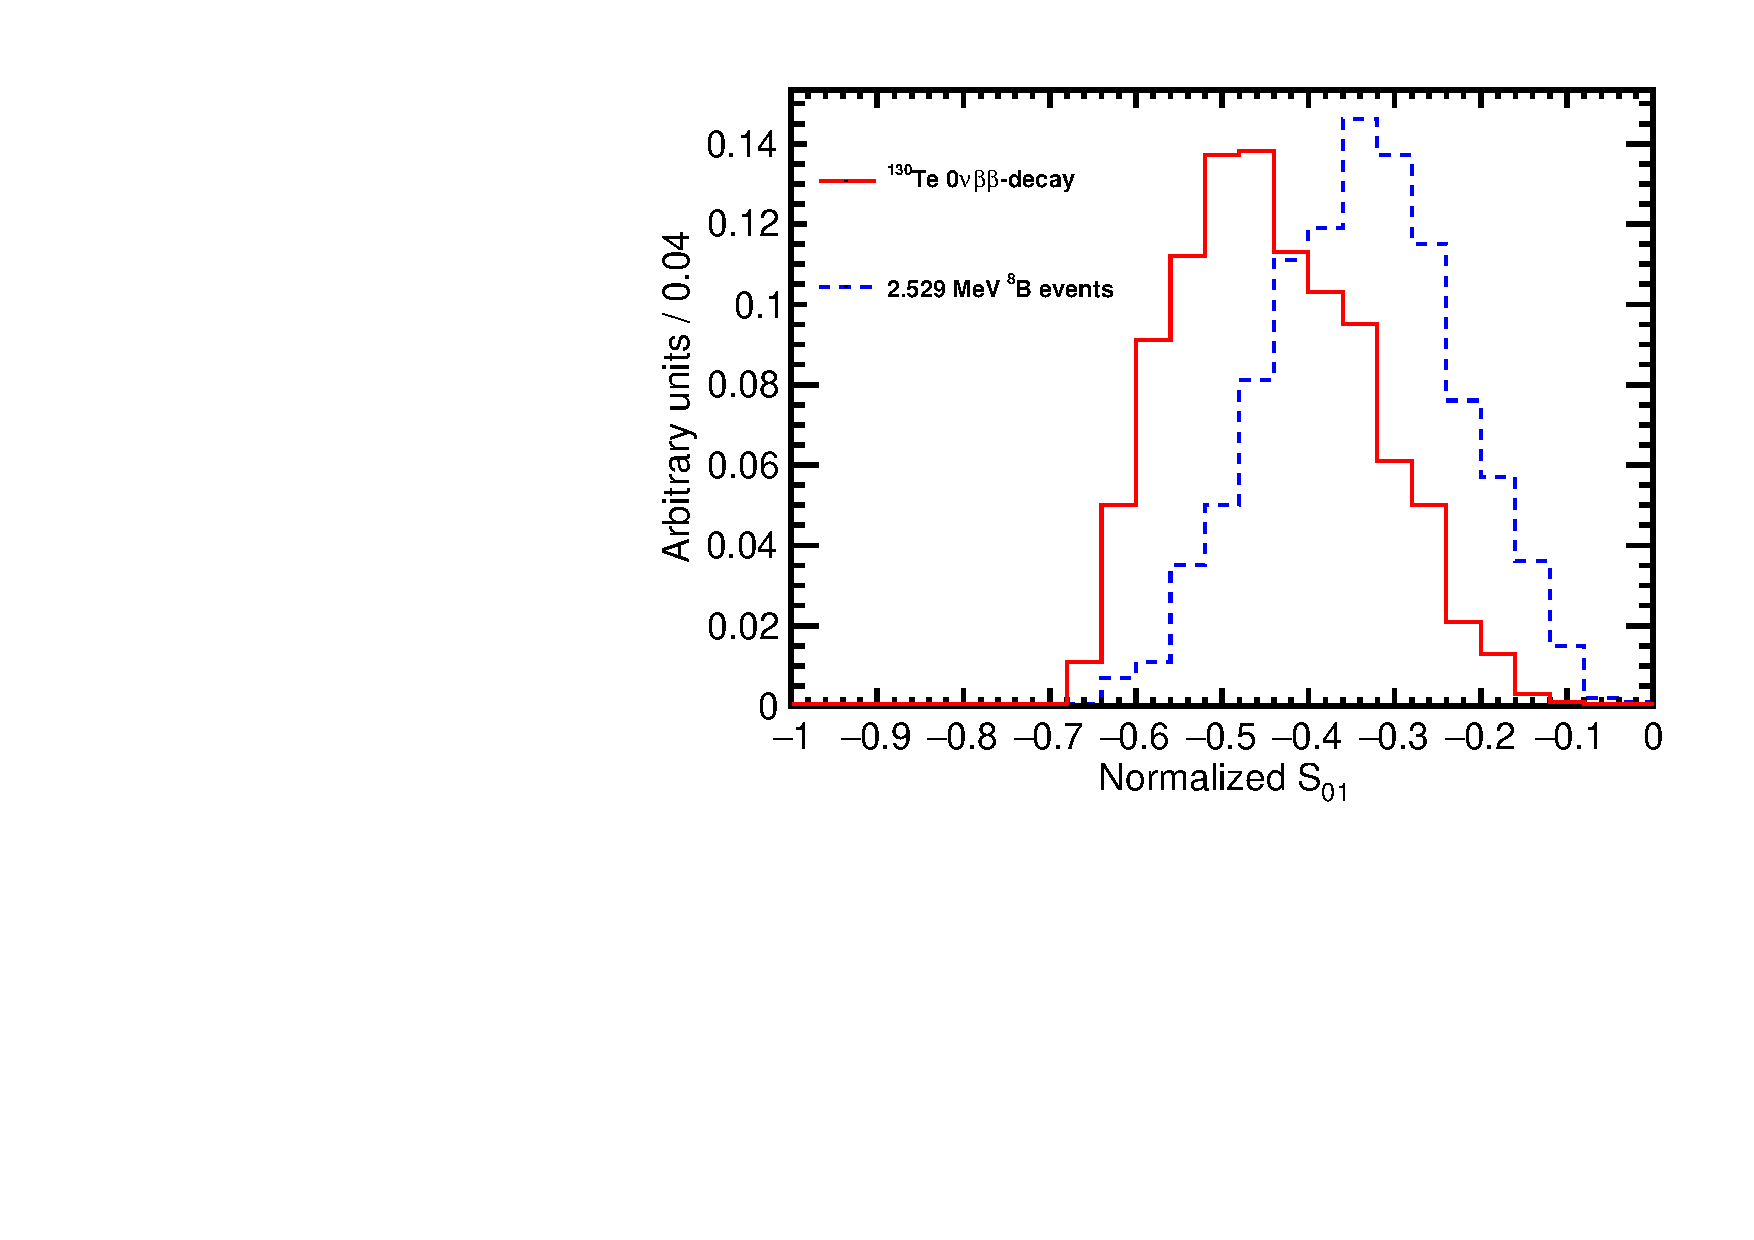
\includegraphics[width=0.49\textwidth]{hS01_allLight_VtxSmear3cm_VtxShiftX0cm_momDT1p0ns_rndVtx_3p0mSphere_SciRT5p0ns}
  \caption{Scintillation rise time constant is increased to $\tau_r=$5~ns compared to $\tau_r=$1~ns in the default detector model.
    \emph{Left:} Scatter plot of $S_0$ versus $S_1$ for a simulation of 1000 signal (\emph{red crosses}) and background
    (\emph{blue triangles}) events. Event verticies are uniformly distributed within the fiducial volume, $R<3$~m.
    Vertex is smeared with 3~cm resolution. Differential cut of
    $\Delta t=t^{phot}_{measured} - t^{phot}_{predicted}<$1~ns is applied to select early PE sample.
    The default QE and 100\% photo-coverage is used in the simulation.
    Black dashed line corresponds to a linear fit to define 1-D variable $S_{01}$ (see text for details).
    \emph{Right:} Comparison of the $S_{01}$ distribution between signal (\emph{red solid line}) and background (\emph{blue dashed line}).
    $I_{overlap}$=0.64.}
\label{fig:SL_Te_SmearX3cm_momDT1ns_rndVtx_3p0m_SciRT5p0ns}
\end{figure*}

%separation = 0.665755
%overlap = 0.642643

Furthermore, the effects due to chromatic dispersion can be addressed by using liquid scintillators with a narrower emission spectrum. For example,
such as described in Ref.~\cite{LS_narrow_emission}.


%Start:
%separation = 0.915454
%overlap = 0.521
%power = 1.76

%Middle:
%separation = 0.357271
%overlap = 0.793
%power = 0.45

%Final:
%separation = 0.665755
%overlap = 0.642643
%power = 1.04
